\documentclass[11pt]{article}

\usepackage[margin=1in]{geometry}
\usepackage[T1]{fontenc}
\usepackage{lmodern}
\usepackage{microtype}
\usepackage{xcolor}
\usepackage{booktabs}
\usepackage{array}
\usepackage{longtable}
\usepackage{tabularx}
\usepackage{graphicx}
\usepackage{listings}
\usepackage{tikz}
\usepackage{float}
\usepackage{enumitem}
\usepackage{tcolorbox}
\usetikzlibrary{arrows.meta,positioning,calc,fit,backgrounds}
\usepackage{hyperref}

\graphicspath{{reports/assets/}{assets/}}

\definecolor{heading}{HTML}{1F4E79}
\definecolor{lightgray}{HTML}{F5F7FA}
\definecolor{codeborder}{HTML}{B8C2CC}
\definecolor{success}{HTML}{1B7F4A}
\definecolor{accent}{HTML}{EAF4FF}
\definecolor{warning}{HTML}{A15C00}
\definecolor{ink}{HTML}{18212B}
\definecolor{panel}{HTML}{F7FAFC}
\definecolor{phaseblue}{HTML}{E6F3FF}

\hypersetup{
  colorlinks=true,
  linkcolor=heading,
  citecolor=heading,
  urlcolor=heading
}

\lstdefinestyle{terminal}{
  basicstyle=\ttfamily\small,
  backgroundcolor=\color{lightgray},
  frame=single,
  rulecolor=\color{codeborder},
  breaklines=true,
  columns=fullflexible,
  keepspaces=true,
  showstringspaces=false
}

\lstdefinestyle{code}{
  basicstyle=\ttfamily\footnotesize,
  backgroundcolor=\color{lightgray},
  frame=single,
  rulecolor=\color{codeborder},
  breaklines=true,
  columns=fullflexible,
  keepspaces=true,
  showstringspaces=false
}

\newcommand{\statusdone}{\textcolor{success}{Complete}}
\newcommand{\statusnote}{\textcolor{warning}{Documented}}
\newcommand{\artifact}[1]{\texttt{#1}}

\newtcolorbox{summarybox}{
  colback=phaseblue,
  colframe=heading,
  boxrule=0.8pt,
  arc=2pt,
  left=8pt,
  right=8pt,
  top=7pt,
  bottom=7pt
}

\newtcolorbox{evidencebox}[1]{
  colback=panel,
  colframe=codeborder,
  title=#1,
  fonttitle=\bfseries,
  boxrule=0.6pt,
  arc=2pt,
  left=8pt,
  right=8pt,
  top=7pt,
  bottom=7pt
}

\setlength{\parindent}{0pt}
\setlength{\parskip}{0.55em}
\renewcommand{\arraystretch}{1.17}
\setlist[itemize]{topsep=0.25em,itemsep=0.2em,leftmargin=1.5em}

\begin{document}
\hypersetup{pageanchor=false}

\begin{titlepage}
\centering
\vspace*{0.7cm}
{\Large Operating Systems Project\par}
\vspace{0.35cm}
{\Huge\bfseries Phase 3 Final Submission Report\par}
\vspace{0.35cm}
{\LARGE CPU Scheduling Simulator Mini OS Component\par}
\vspace{0.8cm}

\begin{summarybox}
\begin{tabularx}{0.92\linewidth}{>{\bfseries}p{0.30\linewidth}X}
Project & CPU Scheduling Simulator \\
Phase & Phase 3: Final Submission, complete project delivery \\
Latest starter commit & \artifact{1e348bb} on 2026-05-06 \\
Repository scope & Scheduler simulation, dashboard, reports, tests, fuzz harnesses, and tooling \\
Main implementation & C11 simulator with a no-build browser dashboard in HTML/CSS/JavaScript \\
Primary verification & \artifact{make test} plus sanitizer-enabled Clang test run \\
\end{tabularx}
\end{summarybox}

\vspace{0.8cm}
\begin{tabular}{cccc}
\toprule
\textbf{Schedulers} & \textbf{C Test Suites} & \textbf{Python Tests} & \textbf{Dashboard} \\
\midrule
7 & 11 & 8 passing & Interactive, screenshot-backed \\
\bottomrule
\end{tabular}

\vfill
{\large Generated from the repository report source on \today\par}
\end{titlepage}

\hypersetup{pageanchor=true}
\pagenumbering{roman}
\tableofcontents
\newpage
\pagenumbering{arabic}

\section{Final Submission Checklist}

This Phase 3 submission is the complete, polished version of the CPU scheduling
simulator proposed for the Operating Systems project. The project focuses on the
CPU scheduler component of a mini operating system: it models process arrival,
burst time, priority, ready-queue decisions, CPU idle periods, context-switch
overhead, Gantt timelines, and scheduler performance metrics.

\begin{evidencebox}{Final submission evidence}
The report was updated from the latest repository commit,
\artifact{1e348bb upgrade report to phase 3 and fix scheduler CSV labels}.
The final verification used the current source tree, regenerated CSV/HTML
evidence, and refreshed dashboard screenshots from a live local browser session.
\end{evidencebox}

\begin{longtable}{p{0.30\linewidth}p{0.18\linewidth}p{0.43\linewidth}}
\toprule
\textbf{Phase 3 Requirement} & \textbf{Status} & \textbf{Evidence} \\
\midrule
Complete working project & \statusdone & C simulator builds with
\texttt{make}; all seven planned schedulers run from the CLI and the browser
dashboard. \\
All planned features working & \statusdone & FCFS, SJF, RR, Priority, SRTF,
Preemptive Priority, and MLFQ are implemented in C and mirrored in the
dashboard. \\
Proper integration & \statusdone & Input loading, scheduler dispatch, Gantt
timeline generation, metrics, visualization, and CSV export share one data
model. \\
Detailed final report PDF & \statusdone & This source file is the final report
source; it includes design, implementation, testing, screenshots, and future
work. \\
Clean code submission & \statusdone & Source is separated into
\texttt{include/}, \texttt{src/}, \texttt{tests/}, \texttt{dashboard/},
\texttt{scripts/}, \texttt{fuzz/}, \texttt{workloads/}, and \texttt{reports/}. \\
README documentation & \statusdone & \texttt{README.md} documents
requirements, build steps, run commands, workload format, algorithms, tests,
dashboard usage, and grading flow. \\
Screenshots and output evidence & \statusdone & Section~\ref{sec:results}
contains current CLI output summaries, regenerated CSV evidence, and
agent-browser dashboard screenshots. \\
Validation evidence & \statusdone & \texttt{make test} passes all C and Python
tests; an AddressSanitizer/UndefinedBehaviorSanitizer test build also passed. \\
\bottomrule
\end{longtable}

\section{Introduction}

CPU scheduling is one of the most visible responsibilities of an operating
system. It decides which ready process receives CPU time, when a process should
wait, and how policy choices affect response time, fairness, throughput, and
CPU utilization. This project turns those scheduler rules into an executable
simulator so that students can test workloads and see the consequences of each
algorithm.

The final project contains two user-facing interfaces:

\begin{itemize}
  \item a C command-line simulator for reproducible scheduler runs, CSV export,
  and automated tests;
  \item a no-build browser dashboard for interactive demonstration, teaching,
  visualization, and project presentation.
\end{itemize}

\section{Problem Statement and Motivation}

Scheduling algorithms are easy to describe in class but difficult to compare
without a working execution model. A small change in arrival order, quantum,
priority, or context-switch overhead can change waiting time and response time
significantly. Manual calculations are also error-prone, especially for
preemptive algorithms.

The project solves this by providing a deterministic simulator that:

\begin{itemize}
  \item accepts process workloads using the format \texttt{pid arrival burst priority};
  \item runs multiple scheduler policies over the same workload;
  \item produces Gantt timelines and per-process timing fields;
  \item computes aggregate metrics for objective comparison;
  \item exports CSV rows for report generation and later analysis;
  \item provides an interactive dashboard so the system can be demonstrated
  clearly during presentation.
\end{itemize}

\section{System Design}

\subsection{High-Level Architecture}

The final system uses a small layered architecture. The CLI and dashboard are
separate interfaces, but they implement the same scheduling rules and compare
the same metrics.

\begin{center}
\resizebox{\linewidth}{!}{%
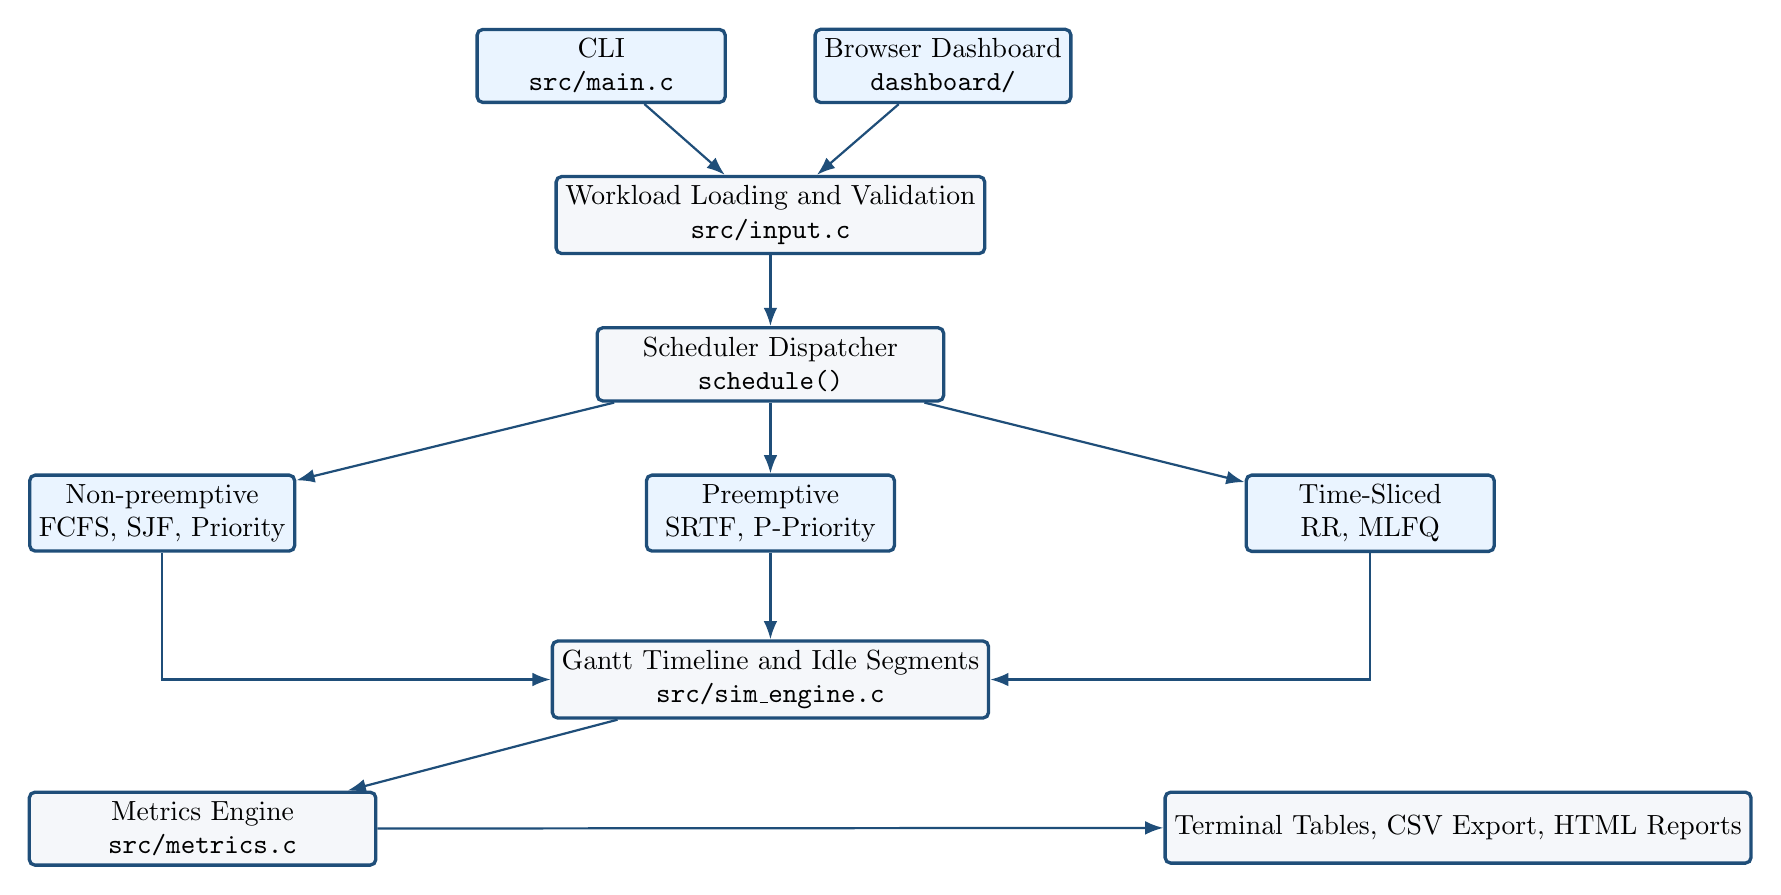
\begin{tikzpicture}[
  node distance=0.9cm and 1.1cm,
  box/.style={
    rectangle,
    rounded corners=2pt,
    draw=heading,
    fill=accent,
    very thick,
    align=center,
    minimum width=3.15cm,
    minimum height=0.9cm
  },
  wide/.style={
    rectangle,
    rounded corners=2pt,
    draw=heading,
    fill=lightgray,
    very thick,
    align=center,
    minimum width=4.4cm,
    minimum height=0.9cm
  },
  arrow/.style={-Latex, thick, draw=heading}
]
\node[box] (cli) {CLI\\\texttt{src/main.c}};
\node[box, right=of cli] (dash) {Browser Dashboard\\\texttt{dashboard/}};
\node[wide, below=of cli, xshift=2.15cm] (input) {Workload Loading and Validation\\\texttt{src/input.c}};
\node[wide, below=of input] (dispatch) {Scheduler Dispatcher\\\texttt{schedule()}};

\node[box, below left=of dispatch, xshift=-2.7cm] (nonpre) {Non-preemptive\\FCFS, SJF, Priority};
\node[box, below=of dispatch] (pre) {Preemptive\\SRTF, P-Priority};
\node[box, below right=of dispatch, xshift=2.7cm] (rr) {Time-Sliced\\RR, MLFQ};

\node[wide, below=1.1cm of pre] (timeline) {Gantt Timeline and Idle Segments\\\texttt{src/sim\_engine.c}};
\node[wide, below left=of timeline, xshift=-1.1cm] (metrics) {Metrics Engine\\\texttt{src/metrics.c}};
\node[wide, below right=of timeline, xshift=1.1cm] (output) {Terminal Tables, CSV Export, HTML Reports};

\draw[arrow] (cli) -- (input);
\draw[arrow] (dash) -- (input);
\draw[arrow] (input) -- (dispatch);
\draw[arrow] (dispatch) -- (nonpre);
\draw[arrow] (dispatch) -- (pre);
\draw[arrow] (dispatch) -- (rr);
\draw[arrow] (nonpre) |- (timeline);
\draw[arrow] (pre) -- (timeline);
\draw[arrow] (rr) |- (timeline);
\draw[arrow] (timeline) -- (metrics);
\draw[arrow] (metrics) -- (output);
\end{tikzpicture}
}
\end{center}

\subsection{Module Explanation}

\begin{longtable}{p{0.28\linewidth}p{0.60\linewidth}}
\toprule
\textbf{Module} & \textbf{Responsibility} \\
\midrule
\texttt{include/} & Public data structures, constants, and module contracts. \\
\texttt{src/main.c} & Parses CLI flags, selects workload input, chooses one
algorithm or all-algorithm comparison, and controls CSV export. \\
\texttt{src/input.c} & Loads built-in samples, workload files, and in-memory
payloads. It rejects duplicate PIDs, invalid times, invalid bursts, malformed
records, extra tokens, and NUL bytes. \\
\texttt{src/process.c} & Initializes process records and resets simulation
state before each algorithm run. \\
\texttt{src/queue.c} & Provides FIFO queue operations and heap-style priority
selection helpers used by schedulers. \\
\texttt{src/sim\_engine.c} & Stores Gantt entries, merges adjacent segments,
tracks idle time, and finalizes total runtime. \\
\texttt{src/schedulers/} & Contains the seven scheduler implementations:
FCFS, SJF, RR, Priority, SRTF, Preemptive Priority, and MLFQ. \\
\texttt{src/metrics.c} & Computes waiting, turnaround, response, CPU
utilization, throughput, context switches, and CSV rows. \\
\texttt{src/visualization.c} & Prints terminal Gantt charts, per-process
tables, aggregate summaries, and all-algorithm comparisons. \\
\texttt{dashboard/} & Static HTML/CSS/JavaScript dashboard with editable
workloads, Gantt playback, metrics cards, comparison charts, race mode,
interactive quiz, and kiosk mode. \\
\texttt{scripts/} & Includes CSV-to-HTML report generation and a local process
logger that can turn observed CPU activity into simulator workloads. \\
\texttt{fuzz/} & AFL++ harnesses, dictionaries, and seed corpora for parser and
queue robustness testing. \\
\bottomrule
\end{longtable}

\section{Implementation Details}

\subsection{Input Model}

Each workload line uses exactly four integer fields:

\begin{lstlisting}[style=code]
pid arrival burst priority
\end{lstlisting}

The validation rules are:

\begin{itemize}
  \item PID must be positive and unique;
  \item arrival time must be non-negative;
  \item burst time must be positive;
  \item priority must be non-negative;
  \item lower priority number means higher scheduling priority.
\end{itemize}

The simulator can load a workload from a file with \texttt{-f} or from a
compiled-in sample with \texttt{-s basic}, \texttt{-s rr},
\texttt{-s priority}, \texttt{-s edge}, or \texttt{-s mixed}.

\subsection{Implemented Scheduling Algorithms}

\begin{longtable}{p{0.22\linewidth}p{0.15\linewidth}p{0.52\linewidth}}
\toprule
\textbf{Algorithm} & \textbf{CLI Key} & \textbf{Final Behavior} \\
\midrule
First-Come, First-Served & \texttt{fcfs} & Non-preemptive. Sorts by arrival
time, then PID, and runs each process to completion. \\
Shortest Job First & \texttt{sjf} & Non-preemptive. Selects the arrived
process with the shortest burst; ties use burst, arrival, then PID. \\
Round Robin & \texttt{rr} & Preemptive by quantum. Uses a FIFO ready queue and
requeues unfinished processes after arrivals from the current quantum are
added. \\
Priority & \texttt{priority} & Non-preemptive. Selects the lowest priority
number; ties use arrival, then PID. \\
Shortest Remaining Time First & \texttt{srtf} & Preemptive SJF. At each event,
selects the ready process with the shortest remaining time. \\
Preemptive Priority & \texttt{priorityp} & Preempts when a higher-priority
process arrives; ties use arrival, then PID. \\
Multilevel Feedback Queue & \texttt{mlfq} & Three queues. New arrivals enter
Q0; processes that consume a quantum are demoted; lower queues use longer or
FCFS-style execution. \\
\bottomrule
\end{longtable}

All seven schedulers now apply \texttt{ctx\_overhead}. When execution switches
to a different PID, the simulator inserts an idle Gantt segment equal to the
configured overhead. This lets the project demonstrate the cost of context
switching, not only the logical order of process execution.

\subsection{Metrics}

The simulator computes the standard CPU scheduling metrics:

\begin{lstlisting}[style=code]
turnaround = completion - arrival
waiting    = turnaround - burst
response   = first_start - arrival
util       = busy_time / total_time
throughput = completed_processes / total_time
\end{lstlisting}

The aggregate metrics are exported to CSV with one row per algorithm, so the
same run can be visualized in terminal output, the browser dashboard, or the
standalone HTML report generator.

\section{Tools and Technologies}

\begin{longtable}{p{0.27\linewidth}p{0.60\linewidth}}
\toprule
\textbf{Tool} & \textbf{Use in Project} \\
\midrule
C11 and \texttt{make} & Main simulator implementation, deterministic tests,
and final build flow. \\
Python 3 and \texttt{pytest} & Helper script tests and CSV report validation. \\
HTML, CSS, JavaScript & No-build dashboard that reimplements the scheduler
rules for live visualization. \\
AFL++ harnesses & Fuzz targets for parser and queue robustness campaigns. \\
Clang sanitizers & AddressSanitizer and UndefinedBehaviorSanitizer validation
used during final verification. \\
TinyTeX and \texttt{latexmk} & Local LaTeX toolchain used for report PDF
generation. \\
\texttt{agent-browser} & Browser automation used to open the live dashboard
and capture final screenshots for this report. \\
CSV visualizer script & \path{scripts/visualize_runs.py} converts simulator
CSV exports into a standalone HTML report. \\
\bottomrule
\end{longtable}

\section{Results and Testing}
\label{sec:results}

\subsection{Automated Test Results}

The final verification run used the documented Python dependencies inside a
local virtual environment:

\begin{lstlisting}[style=terminal,caption={Final command: venv-backed make test}]
PATH="$PWD/.venv/bin:$PATH" make test
test_process: 19/19 passed
test_queue:   22/22 passed
test_input:   22/22 passed
test_fcfs:    19/19 passed
test_sjf:     17/17 passed
test_rr:       9/9 passed
test_priority:13/13 passed
test_srtf:    All SRTF tests passed
test_priority_p: All Preemptive Priority tests passed
test_mlfq:    All MLFQ tests passed
test_metrics: 13/13 passed
pytest tests_py: 8 passed
\end{lstlisting}

A second verification pass built the project with Clang
AddressSanitizer and UndefinedBehaviorSanitizer enabled, then ran the same
\texttt{make test} flow successfully. This provides memory-error and undefined
behavior coverage beyond normal unit-test assertions.

\subsection{Algorithm Comparison Output}

The following comparison was produced from:
\texttt{./cpu\_scheduler -s basic -a all}.

\begin{center}
\begin{tabular}{lrrrrrr}
\toprule
\textbf{Algorithm} & \textbf{Wait} & \textbf{Turn} & \textbf{Resp} &
\textbf{Util} & \textbf{Thr} & \textbf{Ctx} \\
\midrule
FCFS & 8.75 & 15.25 & 8.75 & 1.00 & 0.15 & 0 \\
SJF & 7.75 & 14.25 & 7.75 & 1.00 & 0.15 & 0 \\
RR & 12.75 & 19.25 & 2.00 & 1.00 & 0.15 & 12 \\
Priority & 7.75 & 14.25 & 7.75 & 1.00 & 0.15 & 0 \\
SRTF & 6.50 & 13.00 & 4.25 & 1.00 & 0.15 & 4 \\
Preemptive Priority & 6.50 & 13.00 & 4.25 & 1.00 & 0.15 & 4 \\
MLFQ & 13.00 & 19.50 & 1.50 & 1.00 & 0.15 & 9 \\
\bottomrule
\end{tabular}
\end{center}

\begin{figure}[H]
  \centering
  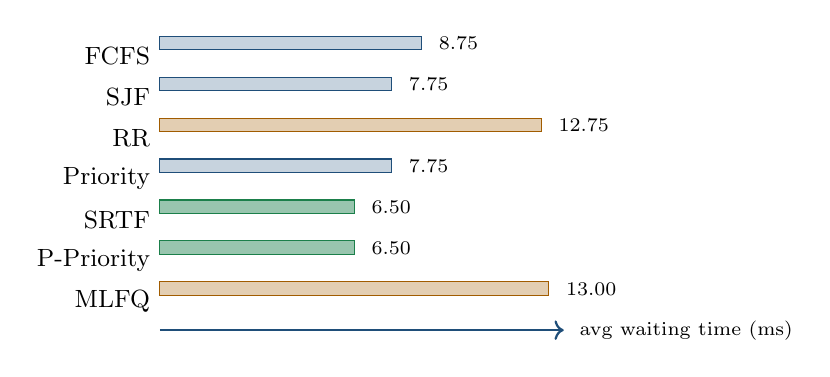
\begin{tikzpicture}[x=0.38cm,y=0.52cm]
    \node[anchor=east,font=\small] at (0,0) {FCFS};
    \draw[fill=heading!25,draw=heading] (0,0.15) rectangle (8.75,0.48);
    \node[anchor=west,font=\scriptsize] at (9.0,0.31) {8.75};

    \node[anchor=east,font=\small] at (0,-1) {SJF};
    \draw[fill=heading!25,draw=heading] (0,-0.85) rectangle (7.75,-0.52);
    \node[anchor=west,font=\scriptsize] at (8.0,-0.69) {7.75};

    \node[anchor=east,font=\small] at (0,-2) {RR};
    \draw[fill=warning!30,draw=warning] (0,-1.85) rectangle (12.75,-1.52);
    \node[anchor=west,font=\scriptsize] at (13.0,-1.69) {12.75};

    \node[anchor=east,font=\small] at (0,-3) {Priority};
    \draw[fill=heading!25,draw=heading] (0,-2.85) rectangle (7.75,-2.52);
    \node[anchor=west,font=\scriptsize] at (8.0,-2.69) {7.75};

    \node[anchor=east,font=\small] at (0,-4) {SRTF};
    \draw[fill=success!45,draw=success] (0,-3.85) rectangle (6.50,-3.52);
    \node[anchor=west,font=\scriptsize] at (6.75,-3.69) {6.50};

    \node[anchor=east,font=\small] at (0,-5) {P-Priority};
    \draw[fill=success!45,draw=success] (0,-4.85) rectangle (6.50,-4.52);
    \node[anchor=west,font=\scriptsize] at (6.75,-4.69) {6.50};

    \node[anchor=east,font=\small] at (0,-6) {MLFQ};
    \draw[fill=warning!30,draw=warning] (0,-5.85) rectangle (13.00,-5.52);
    \node[anchor=west,font=\scriptsize] at (13.25,-5.69) {13.00};

    \draw[->,thick,heading] (0,-6.7) -- (13.5,-6.7);
    \node[anchor=west,font=\scriptsize] at (13.7,-6.7) {avg waiting time (ms)};
  \end{tikzpicture}
  \caption{Average waiting-time comparison for the basic workload. Lower
  values are better; SRTF and Preemptive Priority are the best performers for
  this input.}
\end{figure}

For this workload, SRTF and Preemptive Priority produce the lowest average
waiting and turnaround times. MLFQ gives the fastest first response, while
Round Robin improves response compared with non-preemptive policies at the
cost of more context switches.

\subsection{CSV Export Evidence}

The command below generated
\texttt{reports/assets/phase3\_agent\_browser\_results.csv} with correct
labels and workload descriptors for every algorithm:

\begin{lstlisting}[style=terminal]
./cpu_scheduler -s basic -a all -e reports/assets/phase3_agent_browser_results.csv
.venv/bin/python scripts/visualize_runs.py \
  reports/assets/phase3_agent_browser_results.csv \
  -o reports/assets/phase3_agent_browser_results.html
\end{lstlisting}

\begin{lstlisting}[style=terminal,caption={CSV rows generated by the final simulator}]
algo,n_procs,avg_burst,std_burst,avg_arrival_gap,max_priority,quantum,ctx_overhead,avg_waiting,avg_turnaround,avg_response,cpu_utilization,throughput,context_switches
fcfs,4,6.500000,2.061553,1.000000,4,0,0,8.750000,15.250000,8.750000,1.000000,0.153846,0
sjf,4,6.500000,2.061553,1.000000,4,0,0,7.750000,14.250000,7.750000,1.000000,0.153846,0
rr,4,6.500000,2.061553,1.000000,4,2,0,12.750000,19.250000,2.000000,1.000000,0.153846,12
priority,4,6.500000,2.061553,1.000000,4,0,0,7.750000,14.250000,7.750000,1.000000,0.153846,0
srtf,4,6.500000,2.061553,1.000000,4,0,0,6.500000,13.000000,4.250000,1.000000,0.153846,4
priorityp,4,6.500000,2.061553,1.000000,4,0,0,6.500000,13.000000,4.250000,1.000000,0.153846,4
mlfq,4,6.500000,2.061553,1.000000,4,2,0,13.000000,19.500000,1.500000,1.000000,0.153846,9
\end{lstlisting}

\subsection{Dashboard Screenshots}

\begin{figure}[H]
  \centering
  \IfFileExists{reports/assets/dashboard_phase3_agent_browser_overview.png}{%
    
\includegraphics[width=0.92\linewidth]{reports/assets/dashboard_phase3_agent_browser_overview.png}
  }{%
    \fbox{\parbox{0.86\linewidth}{Dashboard overview screenshot file not found.}}
  }
  \caption{Live browser dashboard overview after loading the repository basic
  workload. The editable process table, scheduler controls, and run controls
  are visible in one view.}
\end{figure}

\begin{figure}[H]
  \centering
  \IfFileExists{reports/assets/dashboard_phase3_agent_browser_gantt.png}{%
    
\includegraphics[width=0.92\linewidth]{reports/assets/dashboard_phase3_agent_browser_gantt.png}
  }{%
    \fbox{\parbox{0.86\linewidth}{Dashboard Gantt screenshot file not found.}}
  }
  \caption{Live browser dashboard showing the all-algorithm Gantt comparison
  for the same basic workload used in the CLI results.}
\end{figure}

\begin{figure}[H]
  \centering
  \IfFileExists{reports/assets/dashboard_phase3_agent_browser_metrics.png}{%
    
\includegraphics[width=0.92\linewidth]{reports/assets/dashboard_phase3_agent_browser_metrics.png}
  }{%
    \fbox{\parbox{0.86\linewidth}{Dashboard metrics screenshot file not found.}}
  }
  \caption{Live browser dashboard showing aggregate metrics, process execution
  details, and the FCFS baseline values after running all algorithms.}
\end{figure}

\begin{figure}[H]
  \centering
  \IfFileExists{reports/assets/dashboard_phase3_agent_browser_comparison.png}{%
    
\includegraphics[width=0.92\linewidth]{reports/assets/dashboard_phase3_agent_browser_comparison.png}
  }{%
    \fbox{\parbox{0.86\linewidth}{Dashboard comparison screenshot file not found.}}
  }
  \caption{Live browser dashboard comparison chart and summary table. It
  highlights SRTF and Preemptive Priority as the best waiting/turnaround
  performers and MLFQ as the best response-time performer for this workload.}
\end{figure}

\section{Challenges and Solutions}

\begin{longtable}{p{0.31\linewidth}p{0.57\linewidth}}
\toprule
\textbf{Challenge} & \textbf{Solution} \\
\midrule
Keeping comparison mode deterministic & Every scheduler resets process state
before running and uses deterministic tie-breakers based on arrival time and
PID. \\
Correct preemption behavior & SRTF, Preemptive Priority, and MLFQ are
implemented as event-aware schedulers that reconsider execution at arrivals,
completions, and quantum boundaries. \\
Round Robin queue ordering & The ready queue adds newly arrived processes
before requeueing the unfinished running process, matching the documented
project rule. \\
Context-switch overhead & All seven schedulers insert idle Gantt segments when
execution switches to a different PID, so overhead affects both total time and
metrics. \\
Parser robustness & The input parser rejects malformed workloads, extra
tokens, duplicate PIDs, NUL bytes, invalid bursts, and invalid negative fields. \\
Keeping dashboard and C behavior aligned & The dashboard JavaScript mirrors
the documented scheduler rules. The named dashboard presets were aligned with
the repository workload files so CLI examples and browser demonstrations use
the same inputs. \\
Final documentation drift & The final pass updated the report, README-visible
sample list, CSV labels, and tests so submitted documentation matches the
current implementation. \\
\bottomrule
\end{longtable}

\section{Future Improvements}

The project is complete for Phase 3, but these extensions would make it more
advanced:

\begin{itemize}
  \item add optional aging to Priority and MLFQ to reduce starvation;
  \item add a batch workload generator for larger performance studies;
  \item save full AFL++ campaign outputs and crash-replay evidence in a
  dedicated validation folder;
  \item export dashboard sessions as JSON so a presentation demo can be replayed
  exactly;
  \item add more command-line tests for invalid flags and boundary-sized
  workloads.
\end{itemize}

\section{Team Contribution}

\begin{evidencebox}{Contribution source}
The table below is based on the repository Git history and the files touched by
each contributor. Official student IDs are not stored in the repository, so the
report records verifiable contribution areas instead of inventing IDs.
\end{evidencebox}

\begin{longtable}{p{0.24\linewidth}p{0.18\linewidth}p{0.46\linewidth}}
\toprule
\textbf{Contributor} & \textbf{Git Evidence} & \textbf{Contribution} \\
\midrule
MoAlsheqaih / Mohammed Al Sheqaih & 22 commits & Scheduler additions,
dashboard integration, MLFQ and preemptive scheduler work, tests, README, and
Phase 3 report assets. \\
mohdm & 10 commits & Helper scripts, CSV visualization, process logger,
requirements, metrics/visualization code, and earlier report work. \\
RN848 & 7 commits & Dashboard specification/design assets, README/report
iterations, process logger setup, and repository documentation. \\
Abdulrahman Alhendawi & 3 commits & Dashboard UI, Gantt/metrics JavaScript,
styling, and visualization report support. \\
\bottomrule
\end{longtable}

\section{Code Submission and Running Instructions}

\subsection{Requirements}

\begin{itemize}
  \item C compiler with C11 support;
  \item \texttt{make};
  \item Python 3 for helper scripts and Python tests;
  \item optional \texttt{pytest}, \texttt{psutil}, AFL++, and sanitizer-capable
  Clang for extended validation.
\end{itemize}

\subsection{Build and Test}

\begin{lstlisting}[style=terminal]
make
make test-c
python3 -m venv .venv
.venv/bin/pip install -r requirements.txt
.venv/bin/python -m pytest -q tests_py
PATH="$PWD/.venv/bin:$PATH" make test
\end{lstlisting}

For the sanitizer validation used in this report:

\begin{lstlisting}[style=terminal]
make clean
PATH="$PWD/.venv/bin:$PATH" make test CC=clang \
  CFLAGS="-std=c11 -Wall -Wextra -Wpedantic -D_POSIX_C_SOURCE=200809L -Iinclude -fsanitize=address,undefined -fno-omit-frame-pointer -g" \
  LDFLAGS="-lm -fsanitize=address,undefined"
\end{lstlisting}

\subsection{Run the Simulator}

\begin{lstlisting}[style=terminal]
./cpu_scheduler -s basic -a all
./cpu_scheduler -f workloads/sample_rr.txt -a rr -q 4
./cpu_scheduler -s basic -a srtf -o 1
./cpu_scheduler -s mixed -a mlfq -q 2
./cpu_scheduler -s basic -a all -e results.csv
\end{lstlisting}

\subsection{Generate CSV/HTML Evidence}

\begin{lstlisting}[style=terminal]
./cpu_scheduler -s basic -a all -e reports/assets/phase3_agent_browser_results.csv
.venv/bin/python scripts/visualize_runs.py \
  reports/assets/phase3_agent_browser_results.csv \
  -o reports/assets/phase3_agent_browser_results.html
\end{lstlisting}

\subsection{Open the Browser Dashboard}

\begin{lstlisting}[style=terminal]
cd dashboard
python3 -m http.server 8080
\end{lstlisting}

Then open \url{http://localhost:8080}. The dashboard can also be opened
directly from \path{dashboard/index.html}.

\subsection{Generate the PDF Report}

The report was compiled locally with TinyTeX and \texttt{latexmk}. From the
repository root:

\begin{lstlisting}[style=terminal]
latexmk -pdf -interaction=nonstopmode -file-line-error \
  -jobname=phase3_final_report -outdir=reports reports/phase3_final_report.tex
\end{lstlisting}

The generated PDF is \path{reports/phase3_final_report.pdf}.

\section{Conclusion}

The Phase 3 project is a complete CPU scheduling simulator mini OS component.
It includes seven scheduling algorithms, workload validation, reusable process
and queue structures, deterministic Gantt timeline generation, metrics,
terminal output, CSV export, a standalone CSV dashboard generator, an
interactive browser dashboard, fuzzing harnesses, and automated tests. The
final verification passes both normal and sanitizer-enabled test runs, and the
report now documents the final state required for submission.

\end{document}
